%============================ Analysis Document ================================
% define document class
\documentclass[
	a4paper               % paper format
%	,10.5pt               % fontsize
	,BCOR=0mm            % Binding correction
	,bibliography=totoc   % If enabled add bibliography to TOC
	,listof=totoc         % If enabled add lists to TOC
%	,bilingual
	,monolingual
	,twoside=false
]{bfhthesis}              % KOMA-script report

\setcounter{secnumdepth}{4}

\PassOptionsToPackage{hyphens}{url}\usepackage[
	hidelinks,
	pdfusetitle,
]{hyperref}
\usepackage{amsmath}
\usepackage{listings}

\LoadBFHModule{boxes}

\colorlet{punct}{red!60!black}
\definecolor{background}{HTML}{EEEEEE}
\definecolor{delim}{RGB}{20,105,176}
\colorlet{numb}{magenta!60!black}

\lstdefinelanguage{json}{
    basicstyle=\normalfont\ttfamily,
    numbers=left,
    numberstyle=\scriptsize,
    stepnumber=1,
    numbersep=8pt,
    showstringspaces=false,
    breaklines=true,
    frame=lines,
	tabsize=2,
	postbreak=\mbox{\textcolor{red}{$\hookrightarrow$}\space},
    backgroundcolor=\color{background},
    literate=
      {:}{{{\color{punct}{:}}}}{1}
      {,}{{{\color{punct}{,}}}}{1}
      {\{}{{{\color{delim}{\{}}}}{1}
      {\}}{{{\color{delim}{\}}}}}{1}
      {[}{{{\color{delim}{[}}}}{1}
      {]}{{{\color{delim}{]}}}}{1},
}

\lstdefinelanguage{canon}{
    basicstyle=\normalfont\ttfamily,
    numbers=left,
    numberstyle=\scriptsize,
    stepnumber=1,
    numbersep=8pt,
    showstringspaces=false,
    breaklines=true,
    frame=lines,
    backgroundcolor=\color{background},
	postbreak=\mbox{\textcolor{red}{$\hookrightarrow$}\space},
}

\hyphenation{ve-ri-fi-ca-ti-on}

\begin{document}

\frontmatter

\title{Bachelor's Thesis}
\subtitle{Unlinkability of Verifiable Credentials in a practical approach: Report}
\author{Joël Gabriel Robles Gasser}
\institution{Bern University of Applied Sciences}
\department{Engineering and Computer Science}
\institute{Computer Science}
\version{1.0}
\date{June 13, 2024}
\advisor{Prof. Dr. Annett Laube\and Prof. Dr. Reto Koenig}
\expert{Dr. Andreas Spichiger}
\degreeprogram{Bachelor of Science in Computer Science}

%----------------  BFH tile page   -----------------------------------------
\maketitle

\addchap{Abstract}
This thesis focuses on analyzing the unlinkability of verifiable credentials when combined with the BBS signature scheme through practical implementation. Initially, it examines the features and key concepts of verifiable credentials, followed by a detailed exploration of their functionality. Algorithms for signing and verifying verifiable credentials, as well as creating selective disclosure verifiable presentations (VPs), are provided. The security concerns associated with using OpenID Connect for verifiable presentations are also analyzed. The research concludes that the implemented methods achieve the desired unlinkability, with potential future enhancements identified to further improve the unlinkability of verifiable credentials in digital identity systems.


%------------ TABLEOFCONTENTS ----------------
\tableofcontents

%------------ START MAIN PART ----------------
\mainmatter

\chapter{Introduction}
In today's digital world, digital identities are mostly managed by centralized entities, like big corporations or governments. This may be easier for individuals as they don't need to manage their data. As the individuals don't have the control how their data is handled, this approach leads to problems with privacy and security. \\

Self-sovereign Identity (SSI)\cite{self-sovereign-identity} is a concept where individuals can control their digital identity and what data is shared with whom. The idea is to allow those individuals to store their data on their own devices, without centralized entities playing middleman. With the data on the device of the individual, they may selectively disclose information, and thus preserve privacy. Another important aspect of SSI is the unlinkability between presentations, meaning that there is no link back to an individual when different data is presented to different verifying parties. Today's centralized entities always know which page an individual visited or what they bought, as they can link all this information back to one individual. A good example for this are targeted ads, which are based on previously revealed information. \\


\begin{figure}[h]
	\centering
	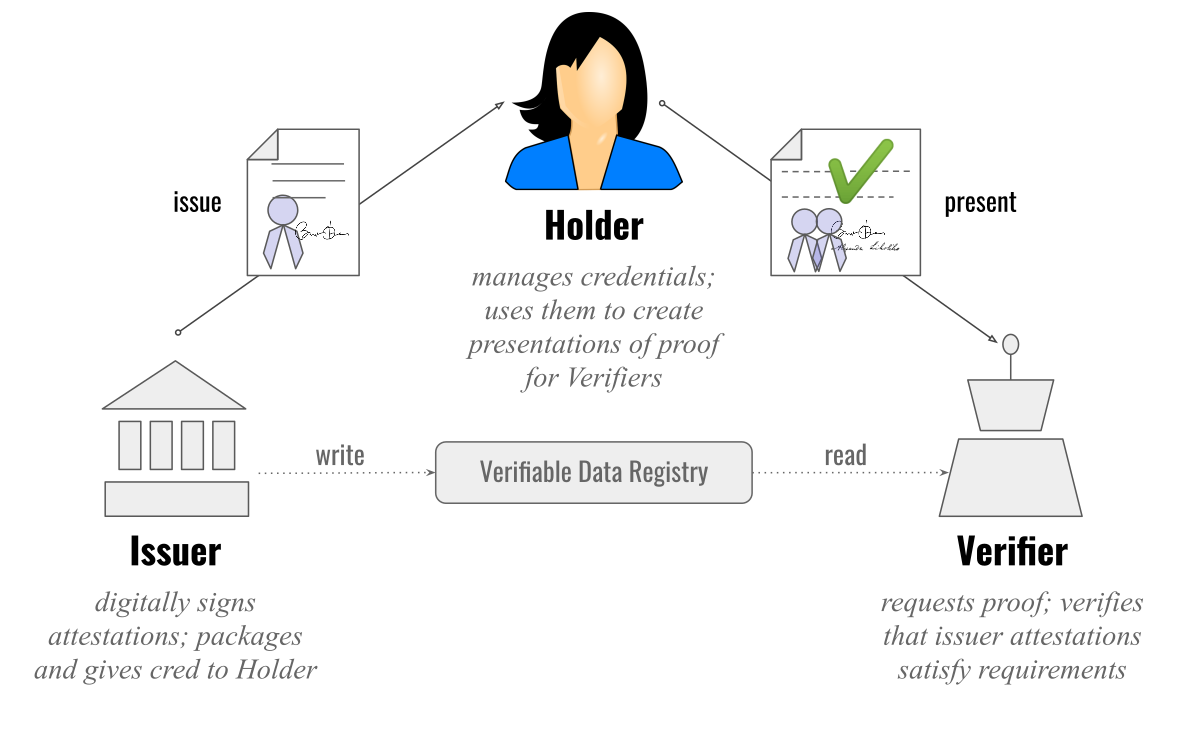
\includegraphics[width=12cm]{./img/trusttriangle.png}
	\caption{The trust triangle\protect\footnotemark}
	\label{fig:trusttringle}
\end{figure}

\footnotetext{\url{https://upload.wikimedia.org/wikipedia/commons/5/51/VC_triangle_of_Trust.svg}}

\newpage
Besides the individual that owns the data, there are more involved entities in SSI, seen in the trust triangle in figure \ref{fig:trusttringle}. The issuer is the entity issuing credentials. A comparison of a credential might be an identity card, which is issued by a state. The third entity is the verifier. This party requests data from a holder, then verifies the response. An example would be the request and the subsequent presentation of a government issued ID when the identity of a holder is challenged. The verifying party is able to trust the presented data, because it is backed by the issuer. For this to work, the issuer must play fair (honest but curious) and does not issue malicious credentials. Only then can the verifier establish trust, hence the name the \textit{trust} triangle. \\

One of the key technologies used in this thesis enabling SSI, is the BBS Signature Scheme (BBS)\cite{bbs-signature-scheme}. This cryptographic signature scheme provides mechanisms for both important SSI features, selective-disclosure and unlinkability. This enables the creation of secure and private verifiable credentials and the digital representation of physical credentials. \\

It is important to understand the difference between physical and digital credentials. First we need to establish that physical credentials can only be used in the physical world, where digital credentials can be used both in the physical and digital world and provide more security and privacy. It is possible that a verifier would accept a physical credential, where all the information that is not needed is taped over, as long as they can verify the validity of the credential (even though one would get weird looks). With that, selective disclosure is achieved. Also, for example when signing a contract, no identifying data is stored by the verifier, as they only check if the individual really is who they say they are. And with that we have the unlinkability. But in the digital world this is different, everything is logged and saved. An individual cannot use their physical credential for a digital interaction. That is why physical credentials need to be translated to digital credentials. Selectively disclosing information gets easier for an individual, when instead of having to change the tape over the hidden information, they can just select what they want to share. But the translation also brings new problems with it. All physical credentials from the same type, like a Swiss government ID, have general security mechanisms, so using those mechanisms for individual verification does not reveal any information. In the digital world, cryptographic signatures are used as a sign of validity, integrity and authenticity of the data. Those signatures are individual per VC. This means that each credential has its own identifier: the signature that is used to protect it. \\

BBS has a solution for this problem. Besides creating the signatures that protect the data and letting the individuals selectively disclose that data, there is a mechanism that allows to randomize the signature, without invalidating it. This allows the verifier to confirm an unlinkable presentation.  \\

The credentials also need to be persisted in some type of construct. In the physical world, it is written on a neat little credit-card sized piece of plastic. That card also has all the security on/in it. In the digital world persistence is usually done with files. These files contain data in a structured way, for example JSON. In our thesis we are using the verifiable credentials data structure (VC)\cite{verifiable-credentials}, a JSON extension. For a holder of a VC it is also easy to store. Instead of adding an ID card to a wallet, a holder adds the persisted VC to a digital wallet on their device. \\

In this thesis we want to investigate the use of the BBS Signature Scheme in a real world scenario.
We assume a working BBS Signature Scheme within the security setting, comprising unlinkability and data integrity.\\

The VCs need to be sent digitally from issuer to holder and presented from a holder to a verifier. 
For this thesis we will only look at the messaging between the holder and the verifier and exclude VC creation and transportation to the holder.
Furthermore we will use an extension of VCs called verifiable presentations (VP)\cite{verifiable-credentials}.
To send a VP between a holder and a verifier, we use OpenID Connect for Verifiable Presentations (OIDC4VP)\cite{oidc4vp}.
We assume secure channels are used for the OIDC4VP communication.\\

Now that we know the different technologies and what they do, we can define the goal of this thesis. We want to analyze if the unlinkability provided by BBS breaks when using it in conjunction with VCs and OIDC4VP in a real world scenario.


\chapter{The BBS Signature Scheme}
The BBS Signature Scheme\cite{bbs-signature-scheme} is a multi-message signature scheme, supporting selective-disclosure and the proof of the knowledge of a signature which in turn creates unlinkability. These features makes this signature scheme an integral part of SSI.\\

\noindent
But what do these features really mean? \\

Normal cryptographic signatures are only able to sign one message at a time, which is viable for digital credentials which contain multiple messages. To sign those credentials; a multi-message signature is needed, which is provided by BBS. The resulting signature provides data integrity for the messages. Important to note is also the fixed size of the signature. No matter the amount and sizes of the messages, the signature length stays the same, thus removing any links between the signature and the signed messages.\\

Now we have a signed set of messages and we would like to present them. All the messages can be presented and verified together using the original signature. The holder may want to only present a sub set of the original messages, selectively disclosing them. To verify a BBS signature, the verifier would need all the data that was signed, so revealing only a part of the data would not work. To be able to that, the holder must generate a new BBS signature, called a BBS proof, which is generated using the original siganture. This new signature is valid for the sub set of the revealed messages with the added protection of proving to the verifier the knowledge of the original signature. This last part is important, as a verifier only trusts the original issuer of a credential and therefore only trusts the original signature.\\

The holder has generated a BBS proof and presented it to a verifier. Now the same holder would like to present the same data to the same verifier again. The easy way would be to use the same proof from the previous presentation. This would create a link to the previous presentation, as the proof value would be an identifier. To prevent the linking of presentations, a new proof must be created for each presentation, as these proofs are random for each generation. With that we have unlinkability between presentations.


\chapter{Use Case}
\label{chap:usecase}
A university issues their diplomas as verifiable credentials to their students. Those contain multiple attributes, like degree, name, university and so on. A student would now like to join an online education platform. Only students with an degree in computer science are allowed to to join the platform.\\

The student can now generate a selectively diclosed VP, which only contains the degree prooving that they studied computer science. All the other attributes stay hidden. The student can now present that VP and is able to join the online course. As each VP is unlinkable because of the BBS proof, the activity of the student stays secret and thus ensures their privacy.


\chapter{Verifiable Credentials and Verifiable Presentations}
\label{chap:vpnvc}
In this chapter, verifiable credentials (VC) and verifiable presentations (VP) are analyzed for data leakage and linkability.
Then we will investigate how we need to manipulate these credentials and presentations, so that they can be signed by the BBS Signature Scheme.

\section{What are VCs and VPs?}
Verifiable credentials\cite{verifiable-credentials} are JSON-LD data models, designed to represent different types of digital credentials.
The idea is to be able to translate physical credentials, like an ID or a driver's license, into the digital world.
These VCs are generated and signed cryptographically by an issuer, like a government.
In this thesis we will use the BBS Signature Scheme to sign the VC.
The content of VC is meta-data, like the life-time or an ID, and an object containing the data that wants to be stored, most of the time, data that belongs to a specific holder.
In the case of a government-issued ID, these can be attributes like birthday, first and last name and so on.
After creation, the issuer sends the VC to the holder.\\

Now the holder would like to present this VC to a verifier.
Using the VC, the holder can generate a verifiable presentation\cite{verifiable-credentials}, which is very close to a VC in structure.
It also contains meta-data that follows the same rules as the meta-data in a VC.
The only difference between a VP and a VC is that a VP contains a whole VC instead of the holder data.
In the case of a VP, we also want to use a cryptographic signature to protect the content against tampering. Here we also use the BBS Signature Scheme.\\

In the next sections we will look at the VC concepts that are used in this thesis.
Please note that there are more concepts, which are out of scope.

\newpage
\section{Used VC concepts}
\label{sec:usedvcconcepts}
In this section we will define all the VC concepts that will be used in this thesis.

\subsection{@context}
The \textbf{@context} attribute is used to map human-friendly IDs like \textit{type} to an URL.
These URLs then help the system understand what the content of the VC is.
The value of the \textbf{@context} attribute is an ordered list, where the first entry must be \textit{\url{https://www.w3.org/ns/credentials/v2}}.\\
We will also use the context \textit{\url{https://w3id.org/security/data-integrity/v2}} to signify that the content of the VC is protected.
Lastly we use a custom context, which describes the content in the credentialSubject.

Our custom context looks like this:
\begin{lstlisting}[language=json,firstnumber=1,caption={Example custom context},captionpos=b]
{
	"@context":{
		"first_name": "https://schema.org/givenName",
		"last_name": "https://schema.org/familyName",
		"birth_date": "https://schema.org/birthDate"
	}
}
\end{lstlisting}

The complete \textbf{@context} which we will use in our example, where the different contexts are represented by URLs, looks like this:
\begin{lstlisting}[language=json,firstnumber=1,caption={Example context},captionpos=b]
{
	"@context": [
		"https://www.w3.org/ns/credentials/v2",
		"https://w3id.org/security/data-integrity/v2",
		"https://raw.githubusercontent.com/robles..."
	],
}
\end{lstlisting}

\subsection{credentialSubject}
\label{subsub:credentialsubject}
The \textbf{credentialSubject} contains a set of objects, which each contain one or more statements about the subject of the credential.\\
In our example we only have one object with three statements about the subject, namely \textit{first\_name}, \textit{last\_name} and \textit{birth\_date}.\\
Such a credentialSubject may look like this:\newpage
\begin{lstlisting}[language=json,firstnumber=1,caption={Example credentialSubject},captionpos=b]
{
	"credentialSubject":{
		"first_name": "John",
		"last_name": "Doe",
		"birth_date": "1.1.1970"
	}
}
\end{lstlisting}

\subsection{ID}
We are also able to add an \textbf{ID} to the VC. This ID can be used to identify a VC or to use it for revocation purposes.\\
There are two places where an \textbf{ID} can be added:
\begin{enumerate}
	\item In the root of the VC, such that the whole VC can be identified
	\item Inside an object of a credentialSubject (see chapter \ref{subsub:credentialsubject}) to identify a specific subject
\end{enumerate}

These IDs must be \textit{URLs} and be either a UUID, a DID or an HTTP URL.

\subsection{type}

The \textbf{type} defines what the context of a VC is. 
It is an array containing either URLs to the description of the VC or can be attributes that must be mapped through \textbf{@context}.
If we use the standard mapped attributes, the type set must either include \textit{VerifiableCredential} or \textit{VerifiablePresentation}.
If we want, we can also add a more specific type, in which we define more information about the VC.\\
In this thesis we won't use any custom types.

\subsection{proof}
\label{subsec:vcproof}
The \textbf{proof} inside a VC guaranties its integrity. But it can also do much more.
In this thesis the proof will either contain a BBS Signature, which signs the VC and with that guaranties its integrity, or it contains a BBS proof, which enables selective disclosure and unlinkability between holder and verifier.\\
The proof object contains following key-value pairs:
\begin{itemize}
	\item \textbf{type}: The type of the proof. In this thesis we use the type \textit{DataIntegrityProof}, as it defines that the proof is there to protect the integrity of the data
	\item \textbf{cryptosuite}: Which cryptosuite was used. In this thesis we use \textit{bbs-2023}, as we use the BBS Signature Scheme
	\item \textbf{created}: A timestamp when the proof was created
	\item \textbf{verificationMethod}: Which verification method is used. This value must be a string that maps to a URL. In this thesis we will use a URL to a public key
	\item \textbf{proofPurpose}: The purpose of the proof. There are two different valid values for this attribute: \textit{assertionMethod} and \textit{authentication}. In this thesis we will use \textit{assertionMethod}
	\item \textbf{proofValue}: The proof value. In this thesis this is either a BBS signature or proof
\end{itemize}

\section{VCs and BBS}
This section contains all the different algorithms to sign a VC, derive a new VC which is used for presentation, create a BBS proof based on the derived VC, wrap the VC in a VP, present it and finally to verify the selectively disclosed VP.\\

In chapter \ref{sec:usedvcconcepts} we defined all the different VC/VP concepts that will be used in this thesis. With that information, we can now build an example VC, that we will use to demonstrate the results of the algorithms.\\
The VC that we will use looks like this:
\begin{lstlisting}[language=json,firstnumber=1,caption={Example VC},captionpos=b,label={list:example-vc}]
{
	"@context": [
		"https://www.w3.org/ns/credentials/v2",
		"https://w3id.org/security/data-integrity/v2",
		"https://raw.githubusercontent.com/robles..."
	],
	"type":  ["VerifiableCredential"],
	"credentialSubject":{
		"first_name": "John",
		"last_name": "Doe",
		"birth_date": "1.1.1970"
	}
}
\end{lstlisting}

\subsection{Sign a VC}
The first step in the process is to sign a VC.
These algorithms are normally called by an issuer, which generated the VC.
As the next step we define some variables, that will be used as the inputs to our algorithms:\\
\textbf{vc}: The VC document, see listing \ref{list:example-vc}\\
\textbf{hmac\_key}: A 32-byte random string, which is used to initialize a HMAC\\
\textbf{verification\_method}: The URL to the verification method\\
\textbf{mandatory\_attributes}: A set of attributes which are mandatory for the holder to disclose to the verifier. For this example we will set the \textit{first\_name} as mandatory. This looks like this: ["credentialSubject/first\_name"]\\

We now define the main algorithm, which calls the sub-algorithms and handles the data between them:
\begin{enumerate}
	\item Set \textbf{proof\_config} and \textbf{canonical\_proof\_config} to the respective entry in the result of the algorithm described in chapter \ref{subsec:proof_config}, with the inputs \textbf{vc.@context} and \textbf{verification\_method}
	\item Set \textbf{transformed\_document} to the result of the algorithm described in chapter \ref{sub:transformvc}, with the inputs \textbf{vc}, \textbf{mandatory\_attributes} and \textbf{hmac\_key}
	\item Set \textbf{hash\_data} to the result of the algorithm described in chapter \ref{subsec:proofHash}, with the inputs \textbf{canonical\_proof\_config} and \textbf{transformed\_document}
	\item Set \textbf{base\_proof} to the result of the algorithm described in chapter \ref{subsec:signvc}, with the inputs \textbf{hash\_data} and \textbf{mandatory\_attributes}
	\item Set \textbf{signed\_vc} to the result of the algorithm described in chapter \ref{subsubsec:addsig}, with the inputs \textbf{vc}, \textbf{proof\_config} and \textbf{base\_proof}
\end{enumerate}

After these steps have the signed VC in \textbf{signed\_vc}.
This algorithm is normally used by issuers, which generate the VC and sign it.
After that, they send the secured VCs to their respective holder, which in turn can use them to create VPs.
Such a signed VC might look like this:
\newpage
\begin{lstlisting}[language=json,firstnumber=1,caption={Signed VC},captionpos=b, label={list:signed-vc}]
{
	"@context": [
		"https://www.w3.org/ns/credentials/v2",
		"https://w3id.org/security/data-integrity/v2",
		"https://raw.githubusercontent.com/robles..."
	],
	"type": [
		"VerifiableCredential"
	],
	"credentialSubject": {
		"first_name": "John",
		"last_name": "Doe",
		"birth_date": "1.1.1970"
	},
	"proof": {
		"type": "DataIntegrityProof",
		"cryptosuite": "bbs-2023",
		"created": "2024-05-20T11:40:13.934Z",
		"verificationMethod": "did:key:zUC7D...",
		"proofPurpose": "assertionMethod",
		"proofValue": "u2V0ChdhAWFC..."
	}
}
\end{lstlisting}

In the coming sections we will define all the sub-algorithms used to generate \\\textbf{signed\_vc}.

\subsubsection{Shuffled label map}
\label{sec:shuffledlabelmap}
This algorithm shuffles the content of a canonical ID map, such that nobody without the hmac key knows the original position of the attributes in the VC.\\

The required inputs of this algorithm are a random 32-bit long bit-string named \\\textbf{hmac\_key} which will be used to initialize a \textit{HMAC} and \textbf{canonical\_id\_map} which contains the map.\\

The output is a function called \textbf{label\_map\_factory\_function}, which shuffles canonical id maps.\\

To shuffle the map, we follow these steps:
\begin{enumerate}
	\item Create a function with the name \textbf{label\_map\_factory\_function}, which has one required input named \textbf{canonical\_id\_map}. Add these steps to the function:
	\begin{enumerate}
		\item Initialize \textbf{bnode\_id\_map} to a new map.
		\item For each entry in the \textbf{canonical\_id\_map}, we split them up into \textit{key} and \textit{value}
		\begin{enumerate}
			\item Set \textbf{hmac\_result} to result of a HMAC-digest operation, which was initialized with the \textbf{hmac\_key}, with the input of \textit{value}
			\item Add a new map entry into \textbf{bnode\_id\_map}, where the key is the \textit{key} and the value is \textbf{hmac\_result} encoded in base64-url encoding defined in chapter 5 and 3.2 of RFC 4648\cite{base64}
		\end{enumerate}
		\item Initialize \textbf{hmac\_ids} to the sorted values of \textbf{bnode\_id\_map}
		\item For each entry in \textbf{bnode\_id\_map}, split up into \textit{key} and \textit{value}
		\begin{enumerate}
			\item Concatenate \textbf{b} with index of \textit{value} in \textbf{hmac\_ids}. Set the result of this concatenation as the value of the current entry in \textbf{bnode\_id\_map}
		\end{enumerate}
		\item Return \textbf{bnode\_id\_map}
	\end{enumerate}
	\item Return \textbf{label\_map\_factory\_function}
\end{enumerate}

\subsubsection{Create the proof config}
\label{subsec:proof_config}
This sub algorithm creates the skeleton of the proof config object, which will be appended to the VC.
This object contains the information about the proof to be generated, like what cryptosuite was used, what type of proof it is etc.\\

The required inputs of this algorithm are the URL of the verification information \textbf{verification\_method} and the context of the VC \textbf{@context}.\\

The output of this algorithm is the proof config \textbf{proof\_config} and the canonicalized proof config \textbf{canonical\_proof\_config}.\\

To generate the proof config, we follow these steps:
\begin{enumerate}
	\item Create an empty \textbf{proof\_config} object
	\item Set \textbf{proof\_config.type} to \textit{DataIntegrityProof}
	\item Set \textbf{proof\_config.cryptosuite} to \textit{bbs-2023}
	\item Set \textbf{proof\_config.created} to the current time
	\item Set \textbf{proof\_config.verificationMethod} to the URL of the verification method \textbf{verification\_method}
	\item Set \textbf{proof\_config.@context} to \textbf{@context}
	\item Set \textbf{canonical\_proof\_config} to the canonical representation of the \textbf{proof\_config} using the \textit{Universal RDF Dataset Canonicalization Algorithm}\cite{rdf}
	\item Return an object containing \textbf{proof\_config} and \textbf{canonical\_proof\_config}.
\end{enumerate}

If we follow the instructions, we get a JSON object like this:
\begin{lstlisting}[language=json,firstnumber=1,caption={Example Proof Config},captionpos=b]
{
  type: "DataIntegrityProof",
  cryptosuite: "bbs-2023",
  created: "2024-05-20T14:25:12.540Z",
  verificationMethod: "did:key:zUC7De...",
  proofPurpose: "assertionMethod",
  "@context": [
    "https://www.w3.org/ns/credentials/v2",
    "https://w3id.org/security/data-integrity/v2",
    "https://raw.githubusercontent.com/robles...",
  ],
}
\end{lstlisting}

This object is then canonicalized into this:
\begin{lstlisting}[language=canon,firstnumber=1,caption={Example Proof Config canonicalized},captionpos=b]
_:c14n0 <http://purl.org/dc/terms/created> \"2024-05-20T14:25:12.540Z\"^^<http://www.w3.org/2001/XMLSchema#dateTime> .
_:c14n0 <http://www.w3.org/1999/02/22-rdf-syntax-ns#type> <https://w3id.org/security#DataIntegrityProof> .
_:c14n0 <https://w3id.org/security#cryptosuite> \"bbs-2023\"^^<https://w3id.org/security#cryptosuiteString> .
_:c14n0 <https://w3id.org/security#proofPurpose> <https://w3id.org/security#assertionMethod> .
_:c14n0 <https://w3id.org/security#verificationMethod> <did:key:zUC7De...> .
\end{lstlisting}

Note that \textbf{@context} is missing from the statements.
This is because it is used by the canonicalization algorithm to determine the type of each attribute in the object.\\

After those steps we now have the skeleton of the proof config object and its canonicalized version.

\subsubsection{Transform the VC}
\label{sub:transformvc}
This algorithm transforms a VC into statements, sorted into mandatory and \\non-mandatory ones. These statements then can be used as an input into the BBS signature algorithm.\\

The required inputs are a VC \textbf{vc}, a 32-byte long \textbf{hmac\_key} to initialize an HMAC and a set of mandatory pointers \textbf{mandatory\_attributes}.\\

The output of this algorithm is an object containing the mandatory and the non-mandatory attributes.\\

To generate the statements, we follow these steps:
\begin{enumerate}
	\item Define \textbf{label\_map\_factory\_function} as the function which is returned from \textbf{create\_shuffled\_id\_label\_map\_function} defined in chapter \ref{sec:shuffledlabelmap} with the input \\\textbf{hmac\_key}
	\item Set \textbf{group\_definitions} to a map where \textit{mandatory} is the key and the value is \textbf{mandatory\_attributes}
	\item Set \textbf{groups} to \textit{response.groups} of the \textit{canonicalizeAndGroup} algorithm specified in the \textit{DataIntegrity for ECDSA specification}\cite{ecdsa}, passing the \\\textbf{label\_map\_factory\_function}, \textbf{group\_definitions} and \textbf{vc}
	\item Set \textbf{mandatory} to the value from \textbf{groups.mandatory.matching}
	\item Set \textbf{nonMandatory} to the value from \textbf{groups.mandatory.nonMatching}
	\item Return an object named \textbf{transformed\_data} containing \textit{mandatory} set to \textbf{mandatory} and \textit{nonMandatory} set to \textbf{nonMandatory}
\end{enumerate}

\newpage
This object may look like this:
\begin{lstlisting}[language=json,firstnumber=1,caption={Return object of the VC transformation},captionpos=b]
{
  mandatory: {
	[
		2,
		"_:b0 <https://schema.org/givenName> \"John\" .\n",
	],
	[
		3,
		"_:b1 <http://www.w3.org/1999/02/22-rdf-syntax-ns#type> <https://www.w3.org/2018/credentials#VerifiableCredential> .\n",
  	],
  	[
		4,
		"_:b1 <https://www.w3.org/2018/credentials#credentialSubject> _:b0 .\n",
	]
  },
  nonMandatory: {
	[
		0,
		"_:b0 <https://schema.org/birthDate> \"1.1.1970\" .\n",
	],
	[
		1,
		"_:b0 <https://schema.org/familyName> \"Doe\" .\n",
	]
  },
}
\end{lstlisting}

And with that we transformed the VC into canonical statements that can later be signed by BBS.

\subsubsection{Hash the proof data}
\label{subsec:proofHash}
In this algorithm we hash the proof data. This data contains the information about the proof, but also the mandatory attributes, which must be revealed.
The hashed data then can be used as the header for the BBS Signature operation, and thus ensures that no information about the proof has changed. It also guarantees that all the correct mandatory data is revealed, as the header value must be the same in the sign, sign verify, proof generate and proof verify process.\\

The input for this algorithm is the proof config as canonical statements \\\textbf{canonical\_proof\_config} and a transformed document \textbf{transformed\_data}.\\

The output is an object \textbf{hash\_data} which is a copy of the \textbf{transformed\_data}, the new hashes of the proof and mandatory data.\\

For the hashing, we follow these steps:
\begin{enumerate}
	\item Set \textbf{proof\_hash} to the result of the hashing of \textbf{canonical\_proof\_config} using SHA-256.
	\item Set the \textbf{mandatory\_hash} to the result of the hashing of \\\textbf{transformed\_document.mandatory} using SHA-256. Be aware that mandatory is an array that first needs to be concatenated. In this thesis we don't use any delimiter for concatenation
	\item Initialize \textbf{hash\_data} as a copy of \textbf{transformed\_data}, then add the key-value pairs \textit{proofHash} - \textbf{proof\_hash} and \textit{mandatoryHash} - \textbf{mandatory\_hash}
	\item Return \textbf{hash\_data}
\end{enumerate}

\newpage
After following these steps, we have an object like this:
\begin{lstlisting}[language=json,firstnumber=1,caption={Return object of the VC transformation},captionpos=b]
{
	mandatory: {
	[
		2,
		"_:b0 <https://schema.org/givenName> \"John\" .\n",
	],
	[
		3,
		"_:b1 <http://www.w3.org/1999/02/22-rdf-syntax-ns#type> <https://www.w3.org/2018/credentials#VerifiableCredential> .\n",
		],
		[
		4,
		"_:b1 <https://www.w3.org/2018/credentials#credentialSubject> _:b0 .\n",
	]
	},
	nonMandatory: {
	[
		0,
		"_:b0 <https://schema.org/birthDate> \"1.1.1970\" .\n",
	],
	[
		1,
		"_:b0 <https://schema.org/familyName> \"Doe\" .\n",
	]
	},
	proofHash: [34, 31, 47, 124, 176, 144, ...],
	mandatoryHash: [51, 239, 227, 180, 185, ...]
}
\end{lstlisting}

Now all the data is in the correct format to generate a BBS Signature.

\newpage
\subsubsection{Generate and serialize the signature}
\label{subsec:signvc}
This algorithm generates a BBS Signature using the input data.\\

The inputs for this algorithm are the hashed data \textbf{hash\_data} and a hmac key \textbf{hmac\_key}.\\

To generate the BBS Signature, we follow these steps:
\begin{enumerate}
	\item Set \textbf{proof\_hash}, \textbf{mandatory\_hash}, \textbf{mandatory} and \textbf{non\_mandatory} to the corresponding value in \textbf{hash\_data}
	\item Set \textbf{bbs\_header} to the concatenation of \textbf{proof\_hash} and \textbf{mandatory\_hash}
	\item Set \textbf{bbs\_messages} to the messages in the \textbf{non\_mandatory} array, which are represented as byte arrays encoded with UTF-8
	\item Set \textbf{bbs\_signature} to the result of the BBS signature operation, defined in chapter 3.5.1 of the BBS Signature Scheme\cite{bbs-signature-scheme}, with \textbf{bbs\_header} and \textbf{bbs\_messages} as the inputs
	\item Initialize \textbf{proof\_value} to the BBS proof header bytes 0xd9, 0x5d and 0x02
	\item Set \textbf{components} to an array containing (in this order): \textbf{bbs\_signature}, \textbf{bbs\_header}, \textbf{public\_key}, \textbf{hmac\_key}, \textbf{mandatory\_pointers}
	\item Set \textbf{cbor} to result of the application of the CBOR-encoding\cite{cbor}, where CBOR tagging \textbf{Must NOT} be used
	\item Set \textbf{proof\_value} to the concatenation of \textbf{proof\_value} and \textbf{cbor}
	\item Set \textbf{base\_proof} to the value of the base64-url encoding defined in chapter 5 of \textit{RFC 4648}\cite{base64} but without padding as mentioned in chapter 3.2 of the same RFC
	\item Return \textbf{base\_proof}
\end{enumerate}

\textbf{base\_proof} now contains a valid BBS Signature, generated with the contents of the VC.

\subsubsection{Add signature to VC}
\label{subsubsec:addsig}
This algorithm adds a BBS Signature to the proof object of a VC.\\

The inputs to this algorithm are a VC \textbf{vc}, the base proof \textbf{base\_proof} and a proof config \textbf{proof\_config}.\\

The output of this algorithm is a signed VC \textbf{vc}.\\

To add the proof to a VC, we follow these steps:
\begin{itemize}
	\item Add a new key-value pair \textit{proof} - \textbf{proof\_config} to \textbf{vc}
	\item Add a new key-value pair \textit{proofValue} - \textbf{base\_proof} to \textbf{vc.proof}
	\item Return \textbf{vc}
\end{itemize}

After following these steps we now have a VC signed by BBS as seen in listing \ref{list:signed-vc}.

\subsection{Derive selective disclosure VP}
As a holder of a secured VC, one would like to present that VC to a verifier.
For that we create a verifiable presentation (VP), which in turn is just a VC containing \textit{@context}, \textit{type} and the VC as \textit{verifiableCredential}.
We also want to use the selective disclosure provided by the BBS Signature Scheme, so that we don't need to disclose all the information contained in the VC.
We will use the signed VC seen in listing \ref{list:signed-vc}.\\
In that example we forced the disclosure of the \textit{first\_name}.
We define that we want to reveal the \textit{last\_name}.\\

As the inputs of the algorithms, we define following variables:\\
\textbf{vc}: The VC, \textbf{not containing} the proof object\\
\textbf{base\_proof}: The proof object from the VC\\
\textbf{selective\_pointers}: An array containing pointers on what should be revealed. In this example we also want to reveal the \textit{last\_name}, so the array looks like this: ["/credentialSubject/last\_name"]\\
\textbf{ph}: The presentation header as a byte array. We will define it as an empty array [] for this example\\
\textbf{verification\_method}: The URL to the verification method\\

This algorithm handles all the data for a selective disclosure proof creation.
First, it generates the derived VC, that will be included in the VP.
Then the BBS Proof is created and replaces the original BBS Signature.
Lastly a VP is created, the VC is added and a new BBS proof is generated for the VP.
After all these steps, the VP is ready to be presented.\\

To create the derived VP, we follow these steps:
\begin{enumerate}
	\item Set \textbf{bbs\_proof}, \textbf{label\_map}, \textbf{mandatory\_indexes}, \textbf{selective\_indexes} and \\\textbf{revealed\_document} to their corresponding entry in the response object from the algorithm described in chapter \ref{subsub:createdisclosuredata}, with the inputs \textbf{vc}, \textbf{base\_proof}, \textbf{selective\_pointers} and \textbf{ph}
	\item Set \textbf{new\_proof} to a copy of \textbf{base\_proof}
	\item Replace \textbf{new\_proof.proofValue} with the result of calling the algorithm in chapter \ref{subsub:serializebaseproof}, with the inputs \textbf{bbs\_proof}, \textbf{label\_map}, \textbf{mandatory\_indexes} and \textbf{selective\_indexes}
	\item Set \textbf{revealed\_document.proof} to \textbf{new\_proof}
	\item Create an empty object \textbf{vp}
	\item Add the key-value pair \textit{@context} - \textbf{revealed\_document.@context} to \textbf{vp}
	\item Add the key-value pair \textit{type} - \textbf{["VerifiablePresentation"]} to \textbf{vp}
	\item Create a map with \textbf{verifiableCredential} as the key and an array, with \\\textbf{revealed\_document} as the only entry, as the value
	\item Add \textbf{verifiableCredential} to \textbf{vp}
	\item Set \textbf{proof\_config} and \textbf{canonical\_proof\_config} to the respective entry in the result of the algorithm described in chapter \ref{subsec:proof_config}, with the inputs \\\textbf{revealed\_document.@context} and \textbf{verification\_method}
	\item Add \textbf{proof\_config} to \textbf{vp}
	\item Set \textbf{bbs\_message} to \textbf{vp} as a string
	\item Set \textbf{bbs\_signature} to the result of the BBS signature operation, defined in chapter 3.5.1 of the BBS Signature Scheme\cite{bbs-signature-scheme}, with \textbf{bbs\_message} and the public key stored at \textbf{verification\_method} as the inputs
	\item Add the key-value pair \textit{proofValue} - \textbf{bbs\_signature} to \textbf{vp.proof}
	\item Return \textbf{vp}
\end{enumerate}

\newpage
This derived VP may look like this:
\begin{lstlisting}[language=json,firstnumber=1,caption={Derived VP},captionpos=b]
{
	"@context": [
		"https://www.w3.org/ns/credentials/v2",
		"https://w3id.org/security/data-integrit...",
		"https://raw.githubusercontent.com/ro..."
	],
	"type": [
		"VerifiablePresentation"
	],
	verifiableCredential: {[
		{
			"@context": [
				"https://www.w3.org/ns/credentials/v2",
				"https://w3id.org/security/data-integrity/v2",
				"https://raw.githubusercontent.com/ro..."
			],
			"type": [
				"VerifiableCredential"
			],
			"credentialSubject": {
				"first_name": "John",
				"last_name": "Doe"
			},
			"proof": {
				"type": "DataIntegrityProof",
				"cryptosuite": "bbs-2023",
				"created": "2024-06-09T14:40:03.606Z",
				"verificationMethod": "...",
				"proofPurpose": "assertionMethod",
				"proofValue": "u2V0Dhd..."
			}
		}
	]}
}
\end{lstlisting}

As you can see, \textit{first\_name} and \textit{last\_name} are shown in the VP, but \textit{birth\_date} is not.
This is the version of the VP that will be presented to the verifier.

\subsubsection{Parse the base proof}
\label{subsub:parsebaseproof}
This algorithm parses the BBS signature in the proof object back into its respective components.\\

The input of this algorithm is a proof object \textbf{base\_proof}.\\

The output is an object \textbf{parsed\_base\_proof} containing the parsed base proof values.\\

We follow these steps to parse the base proof:
\begin{enumerate}
	\item Check that the \textbf{base\_proof} start with an \textit{u}, indicating that it is a base64-url encoded string
	\item Set \textbf{decoded\_proof\_value} to the result of the base64-url decoding with no padding as described in \textit{The Base16, Base32, and Base64 Data Encodings}\cite{base64}
	\item Check that \textbf{decoded\_proof\_value} starts with the BBS proof header bytes \textit{0xd9}, \textit{0x5d} and \textit{0x02}
	\item Set \textbf{components} to the CBOR decoding described in \textit{RFC 8949}\cite{cbor}, starting with the fourth byte in \textbf{decoded\_proof\_value}
	\item Set \textbf{base\_proof\_object} to the key-value pairs \textit{bbs\_signature} - \textbf{components[0]}, \\\textit{bbs\_header} - \textbf{components[1]}, \textit{public\_key} - \textbf{components[2]}, \textit{hmac\_key} - \textbf{components[3]} and \textit{mandatory\_pointers} - \textbf{components[4]}
	\item Return \textbf{base\_proof\_object}
\end{enumerate}

\subsubsection{Create disclosure data}
\label{subsub:createdisclosuredata}
This algorithm generates all the data needed to create a selective disclosure proof. It also generates the derived VC.\\

The inputs of this algorithm are a VC \textbf{vc}, the proof containing the signature \textbf{base\_proof}, the selective pointers \textbf{selective\_pointers} and a presentation header \textbf{ph}.\\

The output is an object containing an BBS proof, a label map, mandatory indexes, selective indexes and the document that we want to reveale (the adjusted VC).\\

To generate all this data, we follow these steps:
\begin{enumerate}
	\item Set \textbf{bbs\_signature}, \textbf{bbs\_header}, \textbf{public\_key}, \textbf{hmac\_key} and \textbf{mandatory\_pointers} to their respective value in the response of the algorithm described in chapter \ref{subsub:parsebaseproof}
	\item Define \textbf{label\_map\_factory\_function} as the function which is returned from the \textbf{create\_shuffled\_id\_label\_map\_function} defined in chapter \ref{sec:shuffledlabelmap} with the input \textbf{hmac\_key}
	\item Set \textbf{combined\_pointers} to the concatenation of \textbf{mandatory\_pointers} and \textbf{selective\_pointers}
	\item Set \textbf{group\_definitions} to an object with following key-value pairs: \textit{mandatory} - \textbf{mandatory\_pointers}, \textit{selective} - \textbf{selective\_pointers} and \\\textit{combined} - \textbf{combined\_pointers}
	\item Set \textbf{groups} and \textbf{label\_map} to \textit{response.groups} and \textit{response.labelMap} respectively of the \textit{canonicalizeAndGroup} algorithm specified in the \textit{DataIntegrity for ECDSA specification}\cite{ecdsa}, passing the \textbf{label\_map\_factory\_function}, \textbf{group\_definitions} and \textbf{vc}
	\item Set \textbf{combined\_match} to \textbf{groups.combined.matching}
	\item Set \textbf{mandatory\_match} to \textbf{groups.mandatory.matching}
	\item Set \textbf{combined\_indexes} to the ordered list of \textbf{combined\_match.keys}
	\item Set \textbf{mandatory\_indexes} to an empty array. We want to compute the position of the mandatory indexes in the \textbf{combined\_match} array, so that the verifier knows which indexes were mandatory to reveal
	\item For each key in \textbf{mandatory\_match} find its index in \textbf{combined\_indexes} and add it to \textbf{mandatory\_indexes}
	\item Set \textbf{selective\_match} to \textbf{groups.selective.matching}
	\item Set \textbf{mandatory\_non\_match} to \textbf{groups.mandatory.nonMatching}
	\item Set \textbf{non\_mandatory\_indexes} to the ordered list of \textbf{mandatory\_non\_match.keys}
	\item Set \textbf{selective\_indexes} to an empty array. This time we want to compute the position of the selective indexes in the \textbf{non\_mandatory\_indexes} list. This list will be used for the BBS proof generation process, to define which messages are going to be revealed
	\item For each key in \textbf{selective\_match} find its index in \textbf{non\_mandatory\_indexes} and add it to \textbf{selective\_indexes}
	\item Set \textbf{bbs\_messages} to the values of \textbf{non\_mandatory.values} as byte arrays
	\item Set \textbf{bbs\_proof} to the result of the BBS proof operation defined in chapter 3.5.3 of \textit{The BBS Signature Scheme}\cite{bbs-signature-scheme}, with the input \textbf{public\_key}, \textbf{bbs\_signature}, \textbf{bbs\_header}, \textbf{ph}, \textbf{bbs\_messages} and \textbf{selective\_indexes}
	\item Set \textbf{revealed\_document} to the result of the algorithm described in chapter 3.4.13 of \textit{Data Integrity ECDSA Cryptosuites v1.0}\cite{ecdsa}, with the inputs \textbf{vc} and \\\textbf{combined\_pointers}
	\item Set \textbf{deskolemized\_n\_quads} to the joined string from the \\\textbf{groups.combined.deskolemizedNQuads} array. In this thesis we do not use a delimiter
	\item Set \textbf{canonical\_id\_map} to the result of the JSON-LD canonicalization algorithm with the input \textbf{deskolemized\_n\_quads}
	\item Set \textbf{verifier\_label\_map} to an empty map. This maps the canonical blank node identifiers like \textit{c14n0} from the revealed VC to the blank node identifiers created by the issuer
	\item For each entry in \textbf{canonical\_id\_map}, where key is \textit{key} and the value is \textit{value}:
	\begin{enumerate}
		\item Add an entry to \textbf{verifier\_label\_map} where the key \textit{value} and the value is the entry in \textbf{label\_map} with the key \textit{key}
	\end{enumerate}
	\item Return an object with following key-value pairs: \textit{bbsProof} - \textbf{bbs\_proof}, \textit{verifierLabelMap} - \textbf{label\_map}, \textit{mandatoryIndexes} - \textbf{mandatory\_indexes}, \textit{selectiveIndexes} - \textbf{selective\_indexes} and \textit{revealedDocument} - \textbf{revealed\_document}
\end{enumerate}

\subsubsection{Serialize the proof value}
\label{subsub:serializebaseproof}
This algorithm serializes the BBS proof value.\\

The inputs of this algorithm are a BBS proof \textbf{bbs\_proof}, a label map \textbf{label\_map}, an array of mandatory indexes \textbf{mandatory\_indexes}, an array of selective indexes \textbf{selective\_pointers} and a presentation header \textbf{ph}.\\

The result of this algorithm is the serialized proof value \textbf{proof\_value}.\\

We follow these steps:
\begin{itemize}
	\item Set \textbf{compressed\_label\_map} to the result of calling the algorithm in chapter 3.5.5 of the \textit{Data Integrity ECDSA Cryptosuites v1.0}\cite{ecdsa} with \textbf{label\_map} as the input
	\item Initialize \textbf{proof\_value} as a byte array, where the first three bytes are \textit{0xd9}, \textit{0x5d} and \textit{0x03}
	\item Set \textbf{components} to an array containing (in this order): \textbf{bbs\_proof}, \\\textbf{compressed\_label\_map}, \textbf{mandatory\_indexes}, \textbf{selective\_pointers} and \textbf{ph}
	\item Set \textbf{cbor} to result of the application of the CBOR-encoding\cite{cbor} on the components array, where CBOR tagging \textbf{Must NOT} be used.
	\item Set \textbf{derived\_proof\_value} to the concatenation of \textbf{proof\_value} and \textbf{cbor}
	\item Set \textbf{derived\_proof} to the the base64-url encoding of \textbf{derived\_proof\_value}, as defined in chapter 5 of "RFC 4648"\cite{base64} but without padding as mentioned in chapter 3.2 of the same RFC
	\item Return \textbf{proof\_value}
\end{itemize}

\subsection{Verify derived VP}
\label{subsub:verifyvp}
The VP was presented by a holder to a verifier. 
The verifier now wants to verify the received VP.\\

We define following variable:\\
\textbf{secured\_document}: This is the VC inside the received VP, so \textbf{vp.verifiableCredential}\\

To verify the VP we follow these steps:
\begin{enumerate}
	\item Set \textbf{bbs\_signature} to \textbf{vp.proof.proofValue}
	\item Remove the key-value pair \textbf{vp.proof.proofValue}
	\item Set \textbf{bbs\_message} to \textbf{vp} as a string
	\item Set \textbf{vp\_pk} to the value stored at \textbf{vp.proof.verificationMethod}
	\item Set \textbf{verified\_vp} to the result of the BBS Signature Verification algorithm defined in \textit{The BBS Signature Scheme}\cite{bbs-signature-scheme} with the inputs' \textbf{vp\_pk}, \textbf{bbs\_signature} and \\\textbf{bbs\_message}
	\item If \textbf{verified\_vp} is false, reject the presented VP
	\item Set \textbf{pk} to the value returned when using the URL from \textbf{secured\_document.proof.}\\
	\noindent
	\textbf{verificationMethod}
	\item Set \textbf{unsecured\_document} to the copy of \textbf{secured\_document} but with the \textit{proof} value removed
	\item Set \textbf{proof} to the copy of \textbf{secured\_document.proof}
	\item Set \textbf{bbs\_proof}, \textbf{proof\_hash}, \textbf{non\_mandatory}, \textbf{mandatory\_hash}, \textbf{selective\_indexes}, \textbf{ph} and \textbf{feature\_option} to their respective entries in the result of the algorithm described in chapter \ref{subsub:parseproof}, with \textbf{proof} as the input
	\item Set \textbf{bbs\_header} to the concatenation of \textbf{proof\_hash} and \textbf{mandatory\_hash}
	\item Set \textbf{disclosed\_messages} to the contents of the \textbf{non\_mandatory}, each UTF-8 encoded
	\item Set \textbf{verify} to the result of the BBS Proof Verification algorithm defined in \textit{The BBS Signature Scheme}\cite{bbs-signature-scheme} with the inputs \textbf{pk}, \textbf{bbs\_proof}, \textbf{bbs\_header}, \textbf{ph}, \\\textbf{disclosed\_messages} and \textbf{selective\_indexes}
\end{enumerate}

After running the algorithm, the verifier has the variable \textbf{verify}. If it's \textit{true}, the verifier knows that the VP is valid and was not tampered with.

\subsubsection{Parse Proof Value}
\label{subsub:parseproof}
This algorithm parses the proof value.\\

The input is a proof value \textbf{proof\_value}.\\

The output is a map containing the BBS proof, a label map, the mandatory indexes, the selective indexes, the presentation header and the feature options.\\

We follow these steps:
\begin{enumerate}
	\item Make sure that \textbf{proof\_value} starts with \textit{u}, which indicates that it is a base64-url encoded value with no padding
	\item Set \textbf{decoded\_proof\_value} to the decoding of \textbf{proof\_value}
	\item Make sure that the three first bytes of \textbf{decoded\_proof\_value} are \textit{0xd9}, \textit{0x5d} and \textit{0x03} in that order
	\item Set \textbf{feature\_option} to \textit{baseline}
	\item Set \textbf{components} to the result of the CBOR decoding of the \textbf{decoded\_proof\_value} starting with the fourth byte. The resulting array must have 5 elements
	\item Replace the second object in \textbf{components} with the result of the algorithm in chapter 3.5.6 of \textit{Data Integrity ECDSA Cryptosuites v1.0}\cite{ecdsa}, with the second object of \textbf{components} as input value
	\item Return a map containing the key-value pairs: \textit{bbsProof} - \textbf{components[0]}, \textit{labelMap} - \textbf{components[1]}, \textit{mandatoryIndexes} - \textbf{components[2]}, \textit{selectiveIndexes} - \textbf{components[3]}, \textit{presentationHeader} - \textbf{components[5]} and \textit{featureOption} - \textbf{feature\_option}
\end{enumerate}

\subsubsection{Create Verify data}
\label{subsub:createverifydata}
This algorithm generates the data for the proof verification process.\\

The input of this algorithm are the VP without the proof value \textbf{document}, the proof \textbf{proof}, and the proof without \textit{proofValue} \textbf{proof\_config}.\\

The output of this algorithm is a label map containing the BBS proof, the proof hash, the non mandatory indexes, the mandatory hash, the selective indexes and the feature options.\\

We follow these steps:
\begin{enumerate}
	\item Set \textbf{proof\_hash} to the hashed (using SHA-256) canonical representation of the \textbf{proof\_config} using the \textit{Universal RDF Dataset Canonicalization Algorithm}\cite{rdf}
	\item Set \textbf{bbs\_proof}, \textbf{label\_map}, \textbf{mandatory\_indexes}, \textbf{selective\_indexes}, \textbf{} and \\\textbf{feature\_option} to their respective entries in the result of the algorithm described in chapter \ref{subsub:parseproof} with \textbf{proof} as the input
	\item Set \textbf{label\_map\_factory\_function} to the algorithm in chapter 3.4.3 of \textit{Data Integrity ECDSA Cryptosuites v1.0}\cite{ecdsa}
	\item Set \textbf{nquads} to the result of the algorithm \textit{labelReplacementCanonicalize} described in chapter 3.4.1 of \textit{Data Integrity ECDSA Cryptosuites v1.0}\cite{ecdsa} with the inputs \textbf{document} and \textbf{label\_map\_factory\_function}
	\item Set \textbf{mandatory} and \textbf{non\_mandatory} to an empty array
	\item For each entry in \textbf{nquads}, the key is \textbf{key} and the value is \textbf{value}, separate it into mandatory and non mandatory
	\begin{enumerate}
		\item If \textbf{mandatory\_indexes} contains \textbf{key}, add \textbf{value} to \textbf{mandatory}
		\item Else add \textbf{value} to \textbf{non\_mandatory}
	\end{enumerate}
	\item Set \textbf{mandatory\_hash} to hash of \textbf{mandatory} using SHA-256. We concatenate the elements of the array without a separator
	\item Return a map containing the key-value pairs: \textit{bbsProof} - \textbf{bbs\_proof}, \textit{proofHash} - \textbf{proof\_hash}, \textit{nonMandatory} - \textbf{non\_mandatory}, \textit{mandatoryHash} - \textbf{mandatory\_hash}, \textit{selectiveIndexes} - \textbf{selective\_indexes}, \textit{presentationHeader} - \textbf{ph} and \textit{featureOption} - \textbf{feature\_option}
\end{enumerate}

\section{Security Considerations of VCs}
\label{subsec:vcseccons}
The combination of BBS and VC raises two security questions:
\begin{enumerate}
	\item If we want to use IDs to identify a revoked VC, we run into linkability problems
	\item The RDF canonicalization algorithm creates data leakage which leads to linkability
\end{enumerate}

\subsection{IDs in VCs}
While creating a VC, the issuer might add an ID to the VC to enable revocation.
A verifier can then check if the ID of the VC, which was presented to them, is in the revocation list of the issuer, and thus accept or reject the presentation.\\
But there is a big problem with this.
If the ID is just added to the VC and is revealed to multiple verifiers, they can link the presentations together based on the ID.
With that we would break the unlinkability provided by BBS.\\

To preserve the unlinkability between the presentations, the holder would need to be able to prove that the ID of the VC is not in the revocation list of the issuer.\\

As a solution to that problem, we can use something like ALLOSAUR\cite{allosaur}. 
With this a holder can prove to a verifier that his ID is not in the revocation list, without presenting a unique identifier.
In this thesis we will assume that the concept shown in ALLOSAUR works without compromising unlinkability.
We also won't look at how it works, as this would be out-of-scope for this thesis.

\subsection{RDF canonicalization algorithm}
In the algorithms described in the Analysis Document, we use RDF multiple times to transform the JSON-LD Document into statements. Using this algorithm can lead to data leakage which in turn can lead to linkability.\\

\newpage
Let's look at an example.
We will use the example given in chapter 6.1 of \textit{Data Integrity BBS Cryptosuites v1.0}\cite{bbsvc}:
\begin{lstlisting}[language=canon,firstnumber=1,caption={Example: Sails VC},captionpos=b]
{
	"@context": [
		"https://www.w3.org/ns/credentials/v2",
		{
		"@vocab": "https://windsurf.grotto-networking.com/selective#"
		}
	],
	"type": [
		"VerifiableCredential"
	],
	"credentialSubject": {
		"sails": [
		{
			"size": 5.5,
			"sailName": "Kihei",
			"year": 2023
		},
		{
			"size": 6.1,
			"sailName": "Lahaina",
			"year": 2023
		},
		{
			"size": 7.0,
			"sailName": "Lahaina",
			"year": 2020
		},
		{
			"size": 7.8,
			"sailName": "Lahaina",
			"year": 2023
		}
		]
	}
}
\end{lstlisting}

\newpage
We use the RDF canonicalization algorithm and get these statements:
\begin{lstlisting}[language=canon,firstnumber=1,caption={Example: Sails VC as statements},captionpos=b]
[
	_:c14n0 <https://windsurf.grotto-networking.com/selective#sailName> "Lahaina" .
	_:c14n0 <https://windsurf.grotto-networking.com/selective#size> "7.8E0"^^<http://www.w3.org/2001/XMLSchema#double> .
	_:c14n0 <https://windsurf.grotto-networking.com/selective#year> "2023"^^<http://www.w3.org/2001/XMLSchema#integer> .
	_:c14n1 <http://www.w3.org/1999/02/22-rdf-syntax-ns#type> <https://www.w3.org/2018/credentials#VerifiableCredential> .
	_:c14n1 <https://www.w3.org/2018/credentials#credentialSubject> _:c14n4 .
	_:c14n2 <https://windsurf.grotto-networking.com/selective#sailName> "Lahaina" .
	_:c14n2 <https://windsurf.grotto-networking.com/selective#size> "7"^^<http://www.w3.org/2001/XMLSchema#integer> .
	_:c14n2 <https://windsurf.grotto-networking.com/selective#year> "2020"^^<http://www.w3.org/2001/XMLSchema#integer> .
	_:c14n3 <https://windsurf.grotto-networking.com/selective#sailName> "Kihei" .
	_:c14n3 <https://windsurf.grotto-networking.com/selective#size> "5.5E0"^^<http://www.w3.org/2001/XMLSchema#double> .
	_:c14n3 <https://windsurf.grotto-networking.com/selective#year> "2023"^^<http://www.w3.org/2001/XMLSchema#integer> .
	_:c14n4 <https://windsurf.grotto-networking.com/selective#sails> _:c14n0 .
	_:c14n4 <https://windsurf.grotto-networking.com/selective#sails> _:c14n2 .
	_:c14n4 <https://windsurf.grotto-networking.com/selective#sails> _:c14n3 .
	_:c14n4 <https://windsurf.grotto-networking.com/selective#sails> _:c14n5 .
	_:c14n5 <https://windsurf.grotto-networking.com/selective#sailName> "Lahaina" .
	_:c14n5 <https://windsurf.grotto-networking.com/selective#size> "6.1E0"^^<http://www.w3.org/2001/XMLSchema#double> .
	_:c14n5 <https://windsurf.grotto-networking.com/selective#year> "2023"^^<http://www.w3.org/2001/XMLSchema#integer> .
]
\end{lstlisting}

The data leakage problem arises in one specific case.
Let's say the holder only discloses information about the sails with the size 7.0 and 7.8, so the last two objects of the credentialSubject.\\


Now, the holder receives a new credential, where information about a sail, which has an entry before the disclosed sails (size 7.0 and 7.8), has been changed.
Let's say that the year for the size 6.0 sail has been updated to 2024.
When the RDF algorithm is now run again on the new VC, we get these statements:
\newpage
\begin{lstlisting}[language=canon,firstnumber=1,caption={Example: Updated sails VC as statements},captionpos=b]
[
	_:c14n0 <https://windsurf.grotto-networking.com/selective#sailName> "Lahaina" .
	_:c14n0 <https://windsurf.grotto-networking.com/selective#size> "6.1E0"^^<http://www.w3.org/2001/XMLSchema#double> .
	_:c14n0 <https://windsurf.grotto-networking.com/selective#year> "2024"^^<http://www.w3.org/2001/XMLSchema#integer> .
	_:c14n1 <https://windsurf.grotto-networking.com/selective#sailName> "Lahaina" .
	_:c14n1 <https://windsurf.grotto-networking.com/selective#size> "7.8E0"^^<http://www.w3.org/2001/XMLSchema#double> .
	_:c14n1 <https://windsurf.grotto-networking.com/selective#year> "2023"^^<http://www.w3.org/2001/XMLSchema#integer> .
	_:c14n2 <http://www.w3.org/1999/02/22-rdf-syntax-ns#type> <https://www.w3.org/2018/credentials#VerifiableCredential> .
	_:c14n2 <https://www.w3.org/2018/credentials#credentialSubject> _:c14n5 .
	_:c14n3 <https://windsurf.grotto-networking.com/selective#sailName> "Lahaina" .
	_:c14n3 <https://windsurf.grotto-networking.com/selective#size> "7"^^<http://www.w3.org/2001/XMLSchema#integer> .
	_:c14n3 <https://windsurf.grotto-networking.com/selective#year> "2020"^^<http://www.w3.org/2001/XMLSchema#integer> .
	_:c14n4 <https://windsurf.grotto-networking.com/selective#sailName> "Kihei" .
	_:c14n4 <https://windsurf.grotto-networking.com/selective#size> "5.5E0"^^<http://www.w3.org/2001/XMLSchema#double> .
	_:c14n4 <https://windsurf.grotto-networking.com/selective#year> "2023"^^<http://www.w3.org/2001/XMLSchema#integer> .
	_:c14n5 <https://windsurf.grotto-networking.com/selective#sails> _:c14n0 .
	_:c14n5 <https://windsurf.grotto-networking.com/selective#sails> _:c14n1 .
	_:c14n5 <https://windsurf.grotto-networking.com/selective#sails> _:c14n3 .
	_:c14n5 <https://windsurf.grotto-networking.com/selective#sails> _:c14n4 .
]
\end{lstlisting}

You can see how the ordering is different, and how the blank nodes (\_:c14nx) were assigned differently.
Even if we didn't disclose any information about the two smaller sails before and after the VC update, a verifier could easily deduce that the content of the VC has changed, which is leaking data. Depending on the size of the VC or what was already revealed, this can even lead to linkability.\\

There is an easy solution to this problem.
As an input to the RDF algorithm we need to pass a function, which takes the canonical labels and replaces them with another value.
If we now add a HMAC (using SHA-256) to this function, we can randomize how the canonical label values are replaced each time a VC is created.\\

Note: It was suggested that the possibility to use KMAC with SHA3-256 should be added to the specification. This was declined by the working group on the basis that SHA-256 is more common.


\chapter{OpenID for Verifiable Presentations}
Now that we know how to create and sign VCs/VPs, we want to be able to send them to the other parties.
In this thesis, we will only look at the communication between a holder and a verifier, so how VPs are transmitted.
As the message layer we use OpenID for Verifiable Presentations(OIDC4VP)\cite{oidc4vp}.
The goal of this chapter is to analyze if OIDC4VP leaks data or even breaks linkability.

\section{How does OIDC4VP work?}
OIDC4VP is a very easy to use protocol.
There are just two parties, the holder and the verifier (which can be split up into holder and wallet, but for the sake of simplicity we merge them).
After the initial interaction between a holder and verifier, these two parties can start a new session, present the VP and close the session.

\begin{figure}[h]
	\centering
	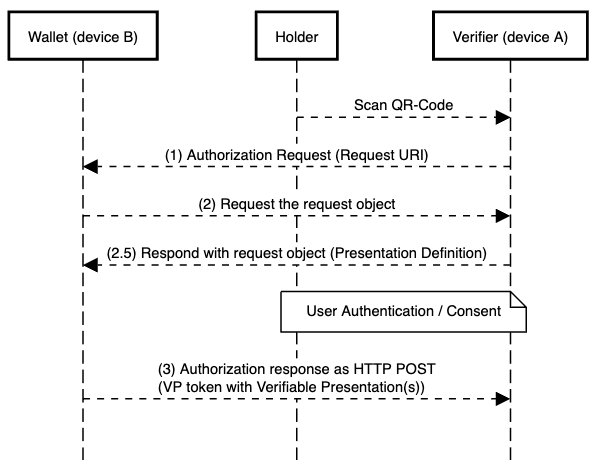
\includegraphics[width=12cm]{./img/oidc4vpflow.png}
	\label{fig:flowvp}
	\caption{Flowchart of OIDC4VP session}
\end{figure}

The flowchart in figure \ref{fig:flowvp} shows the cross-device flow of a OIDC4VP session, meaning the flow, if the initial interaction was not made on the same device, where the VP is saved (for example scanning a QR code from your laptop screen with your phone).\\

In the coming chapters we will examine each step in the session for data leakage and linkability.\\

It's important to note that in this draft, VC and VP can be used interchangeably.
OIDC4VP doesn't really mean that it is only for sending VPs between parties, it is a protocol that defines how the messaging between a holder and a verifier works, independent of VC or VP.\\

\noindent
Also, all the following chapters use HTTP POST/GET requests for the communication.

\subsection{Presentation definition}
\label{subsec:presdef}
The first step in the session is the authorization request. 
In this step the verifier communicates the requirements of the presented VP to the holder, like what type of credential or in which format.
The verifier can also define which individual attributes must be revealed, which is the wanted selective disclosure.

Such an object might look like this:
\begin{lstlisting}[language=json,firstnumber=1,caption={Example of a presentation definition},captionpos=b, label={list:presdef}]
{
	"id": "example with selective disclosure",
	"input_descriptors": [
		{
			"id": "ID card with constraints",
			"format": {
				"ldp_vp": {
					"proof_type": [
						"bbs2023"
					]
				}
			},
			"constraints": {
				"limit_disclosure": "required",
				"fields": [{"path": [
							"$.type"
						],
						"filter": {
							"type": "string",
							"pattern": "IDCardCredential"
						}
					},{"path": [
							"$.credentialSubject.first_name"
						]
					},
				]
			}
		}
	]
}
\end{lstlisting}

Such an object is called \textbf{presentation\_definition}.
There are many new attributes in this object, so let's define them from the top to the bottom. \\

\begin{enumerate}
	\item The \textit{id} in the root is used to identify a specific presentation\_definition. It \textbf{MUST} be present
	\item The \textit{input\_descriptors} is an array describing the different credentials that are requested. It \textbf{MUST} at least contain one entry
	\begin{enumerate}
		\item The \textit{id} inside an input\_descriptor entry is used to identify a specific entry. It \textbf{MUST} be present for each entry in the \textit{input\_descriptors} array
		\item The \textit{format} describes the format of the requested credential. It \textbf{MUST} be present
		\begin{enumerate}
			\item For this thesis we use one of two entries for the \textit{format} object, \textit{ldp\_vc} stating that the requested object must be a VC or \textit{ldp\_vp} stating that it must be a VP.
			\item The \textit{proof\_type} is an array which defines which proof types are accepted. It \textbf{MUST} be present. In this thesis the only proof type that is accepted is \textit{bbs2023}.
		\end{enumerate}
		\item Next we have the \textit{constraints} object. This defines the constraints of the requested credential. It \textbf{MUST} be present
		\begin{enumerate}
			\item If we want to use selective disclosure, we must define \textit{limit\_disclosure} as \textit{required}. If we don't want selective disclosure, \textit{limit\_disclosure} is not present
			\item The \textit{fields} entry is an array which defines which fields must be present, and what the content of those fields might be. It \textbf{MUST} be present
			\begin{enumerate}
				\item The \textit{path} defines the path of a field that must be present. \$ is the root of the presented credential. In listing \ref{list:presdef}, the first entry in the \textit{fields} array defines that the \textbf{type} attribute must be present in the presented credential
				\item If \textit{path} is present we may also use \textit{filter} which lets us filter for specific entries. Again, in listing \ref{list:presdef}, the first entry filters for the type \textit{IDCardCredential} inside the \textbf{type} attribute with \textit{patter}, meaning that \textit{IDCardCredential} must be present. We also define the type of the value, which in this case is a \textit{string}
				\item In the case of selective disclosure, we can also use \textit{path} to define which attributes inside the \textbf{credentialSubject} must be presented. In listing \ref{list:presdef} we define that \textit{\$.credentialSubject.first\_name} must be presented
			\end{enumerate}
		\end{enumerate}
	\end{enumerate}
\end{enumerate}

Now that we know how a presentation definition looks, we can integrate it into the authorization request in two different ways:
\begin{itemize}
	\item Send the whole object as a part of the initial HTTP POST request
	\item Send a \textit{presentation\_definition\_uri} as part of the initial HTTP POST request, which then allows the holder to retrieve the object from a static server
\end{itemize}

But why are there two different integrations?\\
If everything is done on the same device, it is easy to send all the data in the background. But if we are using two devices, we might need to scan a QR Code with the device containing the credential from a second device. There might be the problem that the size of the \textit{presentation\_definition} is too large for a QR Code (max. of 4296 alphanumeric characters).\\

We also want to tell the holder where to send the presentation to.
In this thesis we will use the \textit{direct\_post} response mode, which defines that the response must be sent to an endpoint using an HTTP POST request. The verifier must also set the \textit{response\_uri} parameter with the corresponding uri.

\subsection{Presentation submission}
After the holder got the \textit{presentation\_definition} as well as the \textit{response\_uri} and prepared the VP, he can respond to the verifier.\\

For the response, the holder needs two parameters:
\begin{enumerate}
	\item A \textit{vp\_token} which is just a VP. This VP must be base64-url encoded. It can also be an array of VPs, which each are base64-url encoded
	\item A \textit{presentation\_submission}. This contains a map for the VC inside the VP
\end{enumerate}

\begin{lstlisting}[language=json,firstnumber=1,caption={Example of a presentation submission},captionpos=b, label={list:pressub}]
{
	"id": "Presentation example 1",
	"definition_id": "Example with selective disclosure",
	"descriptor_map": [
		{
			"id": "ID card with constraints",
			"format": "ldp_vp",
			"path": "$",
			"path_nested": {
				"format": "ldp_vc",
				"path": "$.verifiableCredential[0]"
			}
		}
	]
}
\end{lstlisting}

Figure \ref{list:pressub} is an example of a presentation definition. We already know the use of the \textit{id}. The \textit{definition\_id} is just the \text{id} from the \textit{presentation\_definition}.
The \textit{descriptor\_map} is an array that contains the definition for all the VPs inside the \textit{vp\_token}.
In that array we have an \textit{id} for that entry, the \textit{format} of the corresponding credential in the \textit{vp\_token} and the root \textit{path} value.\\
We then have the \textit{path\_nested} object, which contains the \textit{path} of the corresponding credential inside the root credential (like a VC inside a VP) and the   \textit{format} of that credential.\\

To finish the session, the holder just returns the \textit{vp\_token} and the \textit{presentation\_submission} to the verifier.

\section{OIDC4VP Flow}
In this chapter we will look at all the steps between the initial interaction until the verification is complete.
We have 3 entities in this session:
\begin{itemize}
	\item The holder. This entity has the VP that will be presented
	\item The verifier. This entity requests the VP and verifies it
	\item The verifier response endpoint. This entity is a part of the verifier. It receives the VP from the holder and stores it until the verifier requests it
\end{itemize}

The flow between these three parties is shown in the following sequence-diagram:
\begin{figure}[h]
	\centering
	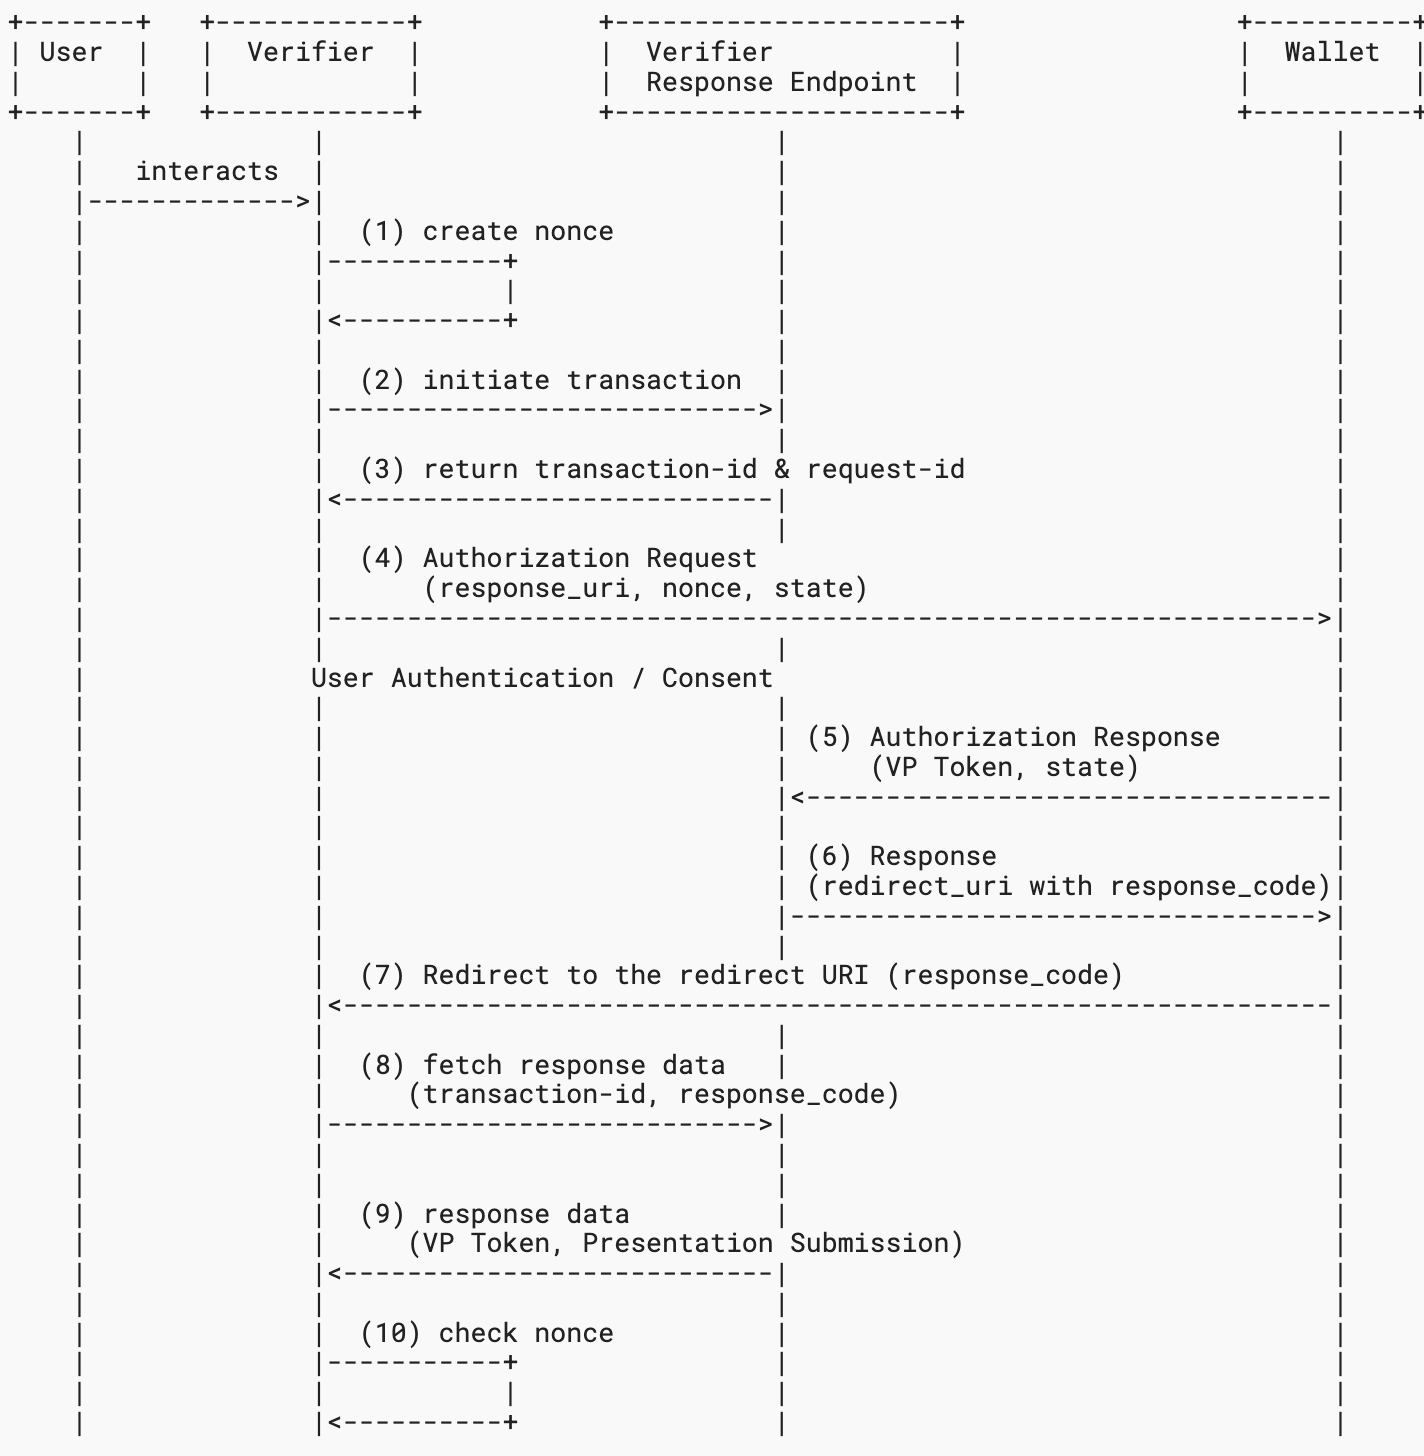
\includegraphics[width=12cm]{./img/oidc4vpflowextended.png}
	\label{fig:flowoid}
	\caption{Full flowchart of a OIDC4VP session}
\end{figure}

With all this information, let's go step by step and look what exactly needs to be done:
\begin{enumerate}
	\item The verifier wants to receive a VP from a holder. The first step is to generate a random number called a \textbf{nonce}. This value is used to counter replay attacks. These attacks try to use data from old sessions and re-submit them to a verifier. With the \textbf{nonce}, the verifier can check if there is an open session connected to it, and if not, the invalid presentation is rejected (Step 1 in figure \ref{fig:flowoid})
	\item The next step is to initiate a transaction between the verifier and the verifier response endpoint. The endpoint responds with two random numbers, the \textbf{transaction\_id} and the \textbf{request\_id}. The endpoint then keeps a map of both values as they belong together. The \textbf{request\_id} is given to the holder, who uses it to tell the endpoint to which session (transaction) the presentation belongs. At the end of the session, a verifier can then fetch the presentation from the endpoint using the \textbf{transaction\_id} (Step 2 and 3 in figure \ref{fig:flowoid})
	\item The verifier now generates a QR code for the holder to scan. In this thesis we will use the response mode \textit{direct\_post}. This mode allows to the holder to send the response to the verifier using a redirect. The QR code must contain the following information (Step 4 in figure \ref{fig:flowoid}):
	\begin{itemize}
		\item \textbf{response\_mode}: In this thesis, we set this value to \textit{direct\_post}
		\item \textbf{response\_uri}: This value contains the uri where the holder need to send the VP to
		\item \textbf{client\_id\_scheme}: This value defines the type of the \textbf{client\_id} value
		\item \textbf{client\_id}: In this thesis, this value must be the same as \textbf{response\_uri}
		\item \textbf{response\_type}: This value defines the type of the response. For OIDC4VP this value must be set to \textit{vp\_token}
		\item \textbf{nonce}: The \textbf{nonce} as defined above
		\item \textbf{state}: The \textbf{request\_id} as defined above
		\item \textbf{presentation\_definition}: The presentation definition as defined in \ref{subsec:presdef}
	\end{itemize}
	\item After scanning the QR code, the holder generates the VP corresponding with the \textbf{presentation\_definition}. It is important to note that there are two special things that the holder needs to add to the VP. First the \textit{nonce} needs to be added in the proof object of the VP. Then the \textit{client\_id} also needs to be added to the proof object, but as the domain. This domain value must also be used by the holder as an input to the BBS proof generation algorithm. This VP is called the \textit{vp\_token}. The holder also generates the \textit{presentation\_submission}. These values are then sent together with the \textbf{state} to the verifier response endpoint defined in \textbf{response\_uri} (Step 5 in figure \ref{fig:flowoid})
	\item The verifier response endpoint receives the response from the holder. Using the \textit{state} (which initially was the \textbf{request\_id}), the endpoint can match the response from the holder to an open transaction with the verifier. Then the endpoint returns a \textit{redirect\_uri} and \textit{response\_code} to the holder. This points the holder back to the verifier to message him that the presentation was sent to the endpoint. The code is again a random number, which is linked to the respective presentation. There would be a possible implementation without this response to the holder. In that implementation the verifier would continuously pull the new data from the endpoint to check if the VP was presented. This would enable a session fixation attack (Step 6 in figure \ref{fig:flowoid})
	\item The holder now has the \textit{redirect\_uri} and \textit{response\_code}. They now send an HTTP POST request to the \textit{redirect\_uri} with the \textit{response\_code} to the verifier. After sending the request, the session is finished for the holder (Step 7 in figure \ref{fig:flowoid})
	\item After receiving the \textit{response\_code} from the holder, the verifier now fetches the \textit{vp\_token} and \textit{presentation\_submission} from the endpoint. For that they send an HTTP POST request containing the \textbf{transaction\_id} and \textbf{response\_code}. The \textit{transaction\_id} is only known by the verifier, but it might be that the system is compromised. As the \textit{response\_code} is only known to the part of the system, where the holder was redirected to, so the compromised part of the system is not able to pull the data of the holder. The endpoint then responds with the corresponding \textit{vp\_token} and \textit{presentation\_submission} (Step 8 and 9 in figure \ref{fig:flowoid})
	\item In the last step, the verifier now verifies the nonce included in the \textit{vp\_token}. If that nonce is correct, they can verify the VP and either accept or reject it (Step 10 in figure \ref{fig:flowoid})
\end{enumerate}

\section{Security concerns}
Adding OIDC4VP to the VC/VP-BBS stack raises two new security concerns:
\begin{itemize}
	\item We want to use nonce to avoid replay attacks
	\item Session fixation attacks are possible if the holder is not re-reouted
\end{itemize}
As all the data is generated randomly, no problems with unlinkability and selective disclosure is created.

\subsection{Replay attacks}
If a holder sends data to a verifier trought a channel that has a middle man in it, a replay attack is possible even if the data is encrypted.
A replay attack is an attack, where data that was already presented once, is presented again to, for example, gain access to an account.
To prevent such attacks, values called \textit{nonce} are used. When a session is created, a \textit{nonce} is given to the holder.
The holder then can present data with that nonce once. After receiving the data, the verifier then removes the nonce from the active list, so that presenting data with the same nonce again is rejected.
A basic way to create a \textit{nonce} is a counter. Using a counter is only secure until the current value is known. To replay already presented data, an attacker would then just need to add a higher value as the current counter.
A more secure version would be to generate random numbers, and then adding those numbers to a active list. When a session is finished, the nonce of that session is removed from that list.

\subsection{Session fixation}
A session fixation attack works when an attacker steals a token from a holder and uses that to keep a session open.
In OIDC4VP a session fixation attack can be used to get the unencrypted data from a presentation.
If attacker infiltrated a verifier, they could get the transaction-id and request-id for a session (see figure \ref{fig:flowoid}).
Using those IDs, the attack could then query the verifier backend to get the response data from the session.
This attack can only happen if steps 6 and 7 in figure \ref{fig:flowoid} are not implemented, thus letting the verifier querying the endpoint until they get a response.\\
To prevent this attack from happening, steps 6 and 7 in figure \ref{fig:flowoid} should be implemented. This adds two security features to the flow.
First a random response code is generated. The verifier and the attacker wouldn't receive the data from the backend with just the transaction-id and request-id, as they would also need the response code. 
If the holder then would just send back the response code to the verifier, the attacker would also have it, which defeats the point of that code. That is why the holder also gets a redirect uri from the endpoint.\\
The holder send the reponse code to the redirect uri, which is in another part of the verifiers system. With that the attacker never has all pieces and thus isn't able to access the presented data.


\chapter{Sandbox}
While researching for the integration of BBS into VCs, I came by the \textit{Data Integrity BBS Cryptosuites v1.0}\cite{bbsvc} specification.
This specification contains all the necessary information about how to process a VC into statements, selectively disclose those statements, sign the VC and then also verify that VC.\\
Sadly, the specification was a bit of a mess (it was updated recently, so it is much better now). That is why I talked with Greg Bernstein, one of the authors of the specification, which linked me to his test implementation. Using that implementation I went through the specification and described all the steps in chapter \ref{chap:vpnvc}. I also used the same implementation to generate all the VCs \& VPs seen in this thesis.\\

If you, the reader, would also like to know how everything works, you can download the library here: \url{test url}.\\

Here some quick tips how to use the library:
\begin{itemize}
	\item All the files that can be changed or run are in the /examples folder
	\item Inside the /examples/input folder there are different files that can be changed. example.json contains the VC structure, mandatory.json the mandatory pointers and selective.json the selective pointers
	\item To run files, cd into the /examples directory and run 'node <filename.js>'
	\item Running createSignedBase.js generates a signed VC, which can be found in the /examples/output folder
	\item Running verifySignedBase.js verifies the generated VC and prints the result in the terminal
	\item Running deriveDocument.js generates a derived VC, using the before generated signed VC and the selective pointers. The derived VC can also be found in the /examples/output folder
	\item Running verifyDerivedDocument.js verifies the derived VC, and prints the result in the terminal
	\item If you want to create a custom context, create a new js file in /examples/contexts. Then import the new file into /examples/documentLoader.js and add the new url to the existing list
\end{itemize}

Do not forget to run 'npm i' in the root folder after downloading the library, to install all dependencies.


\chapter{Future Work}
In the timeframe of this thesis, not all planned technologies were analyzed. These can be part of future works to extend the features of this stack. These features are Blind BBS Signatures, BBS Pseudonyms and Link Secrets. \\

In this thesis, the use case presented in chapter \ref{chap:usecase} is only for demonstrative purposes. We don't yet have a concrete use case, where all the features of the described technologies really show their usefulness. With time, when digitalizing credentials becomes more common, one might find a use case where selective disclosure and unlinkability are very important. \\

An other point for future work would be the implementation and testing. This thesis only contains theoretical analysis of the different technologies. Implementations using different programming languages might create new problems which were not part of this thesis. \\

At last, the communication between an issuer and a holder must be analyzed. OpenID Connect for Verifiable Presentations would be used, but this was excluded from this thesis.


\chapter{Conclusion}
The most important thing to say is that \textbf{it works}! The goal of this thesis, to analyze the inner workings of the different technologies and to find solutions to keep the unlinkability intact, is reached.\\

It was very interesting to research for this project. After learning how BBS works under the hood the semester before for the Project 2 module, learning how to integrate it with other technologies was very interesting and challenging. After setting up the project, looking at the risks and arranging the different sprints and sub-goals for 3 weeks, I was ready to start researching. \\

The first step was to find out how the verifiable credentials work. After reading the VC specification for some time, I encountered two problems. The first problem was the sheer size of the specification. There were so many optional features or different ways to do something that I had to narrow it down. So after sometime testing, I defined a minimal set of features found in chapter \ref{sec:usedvcconcepts}. Based on that I could then create a VC and concentrate on how to add BBS into the mix, which was the second problem. After some research I found the \textit{Data Integrity BBS Cryptosuites v1.0}\cite{bbsvc} specification, which states exactly how to merge both technologies. Problem was, it was not comprehensible. In the time after my research into that topic, the specification was updated and is thus more readable, but it was really hard to understand. That is why I contacted one of the authors of the specification, Greg Bernstein, which referred me to his implementation. Using that implementation I then understood the different steps of the specification and wrote them up. After finishing analyzing all the algorithms, I searched for security problems. Two problems were found, one in the algorithm of the VC transformation (so that the VC could be signed) and a second one regarding identifying meta-data, which were both solved. At the end of the thesis a third problem popped up, but it was not analyzed because of time constraints. This problem is about the signing of a VP. The verifier doesn't trust the holder, so how can the holder sign the VP that he generated. This is something that should be analyzed in future work. \\

After finishing up researching VCs, the next topic was OpenID Connect for Verifiable Presentations. Here again, the first step was to read the specification. This time it was not as extensive as the VC specification, and there were not many different optional features, so it was more straight forward. So after a week of reading and documenting, this step of the process was done. \\

\newpage
After that there was not much time left until the due date, so out of time constraint reasons, the research on Blind BBS Signatures, pseudonyms and link secrets was not done. \\

Another thing besides the messy VC-BBS specification creating time problems, was the documentation. For me, writing is very difficult and takes a lot of time and tries for getting it to an acceptable level. For example the research, documenting and implementation of VCs \& VPs should have only take one week each. In the end it was 3 weeks of research and 4 weeks of testing Greg Bernsteins library and documenting the findings. At the same time I needed to prepare the book entry and the poster, create my defense to make a test presentation with expert and guests and also create the video, the small presentation and prepare the demo day. Each of those assignments took time away from the main task of documenting and thus leaving me with less time than expected. \\

At the end of the day, I'm happy with my results. I've learned a lot of new things about different technologies, but also about researching and documenting. It was a very interesting semester, with a lot of up and downs. I will use the acquired knowledge to implement this technology stack and to keep researching the missing features.\\

A big thanks goes out to my advisors, Laube Annett and Reto Koenig. Dealing with me on a weekly basis must have been tiring. They also really helped me to get throught documenting everything. Also a big thanks to my expert, Andreas Spichiger, who took time to listen to my presentations and give me feedback. This feedback helped me to create a better defense.\\

Also very important are my mother, my sister and my aunt. All these women generously helped me by proof reading the documentation, listening to my presentations and by being my guinea pigs to see if the text was abstract enough. Big thanks to them!\\

Last but not least, big thanks to my girlfriend. Without her i would have probably starved to death. Because of her I got a nice meal each evening, without needing to consume time cooking. Those meals gave me energy to keep going. And also a big thanks for helping me in coming up with ideas on how to explain ceratin things.\\

And on a small side note, also small thanks to myself on not giving up after learning that there is not time to implement something.


\bibliographystyle{plain}
\bibliography{refs}


\end{document}
